% +--------------------------------------------------------------------+
% | Sample Chapter 2
% +--------------------------------------------------------------------+

\cleardoublepage

% +--------------------------------------------------------------------+
% | Replace "This is Chapter 2" below with the title of your chapter.
% | LaTeX will automatically number the chapters.                      
% +--------------------------------------------------------------------+

\chapter{Apparatus}
\label{makereference2}

Two pieces of apparatus were used to conduct the experiments in this thesis. This chapter will detail the purpose, design and recreation of the equipment. Section ~\ref{makereference2.1} will cover the new Motorlab, including the hardware implementation, design of components, and basic functionality. Section ~\ref{makereference2.1.2} will detail how a new type of position sensor works that is used for the position measurements of the Motorlab. Then, the older Motorlab will be discussed and compared to the new Motorlab in section ~\ref{makereference2.2}.

\section{New Motorlab}
\label{makereference2.1} 

The new Motorlab is a reimplementation of older laboratory hardware created by Dr. Schinstock and Dr. White for Control of Mechanical Systems I at Kansas State University. The Motorlab allows users to connect the theoretical ideas of control theory with those in practice. (Maybe include applications of the motorlab and its use in the laboratory).

\subsection{Hardware}
\label{makereference2.1.1} 

The new Motorlab consists of several key pieces of hardware, namely a \ac{MPU}, motor driver, and a \ac{BLDC} motor. The main MPU of the Motorlab is the STM32 Nucleo, which allows Arduino attachment shields and other STM boards to be attached for added functionality. For the purposes of the Motorlab, a motor driver was required to drive a brushless DC motor, namely a [Motor Brand]. An X-Nucleo-IHM07M1 (a three-phase brushless DC motor driver) was selected to be the primary driver for the Motorlab.

\subsection{Position Sensor}
\label{makereference2.1.2} 

The main purpose of the Motorlab is to conduct control laboratory experiments, as a result, feedback via sensor readings is necessary to do such control. The typical way to do position and speed control of mechanical systems and motors is to use position feedback via an encoder. An encoder is a device that converts angular position of a motor shaft to an analog or digital signal that can be processed by an MPU. In the case of the Motorlab, an on-axis magnetic encoder is used to do position feedback. Special equipment had to be designed in order to use this type of encoder, and will be detailed in section ~\ref{makereference2.1.2}.  

The encoder that is being used on the Motorlab consists of 14-bit on-axis magnetic rotary position sensor chip, specifically the AS5047D by AMS \footnote{AMS is an Austrian analog sensor and semi-conductor manufacturer}. The position sensor chip provides high resolution absolute angle measurements through a full 360 degree range \footnote{These chips typically provide a maximum resolution of 2000 steps/revolution in decimal mode and 2048 steps/revolution in binary mode}. In addition to the fast absolute angle measurement system that the position sensor provides, it also has \ac{DAEC} that provides position control systems with near 0 latency \citep{1}.  

The AS5047D chip is a magnetic sensor that utilizes the Hall-effect. The chip works by taking the Hall sensors and converting the perpendicular magnetic field on the surface of the chip to a voltage. The voltage signals are filtered and amplified in order to calculate the angle of the magnetic vector. In order for position measurements to be taken, a small diametrically opposed magnet must be placed on the shaft of the equipment being measured. The magnet and AS5047D are contactless, meaning there is a small air gap between the chip and magnet. As the magnet rotates above the chip (Figure~\ref{magnet_rotation}), angle measurements are calculate and transmitted through the chip \citep{1}. The Motorlab uses the AS5047D chip primarily as a position and speed control system. 

\begin{figure}[htb]%t=top, b=bottom, h=here
\begin{center}
    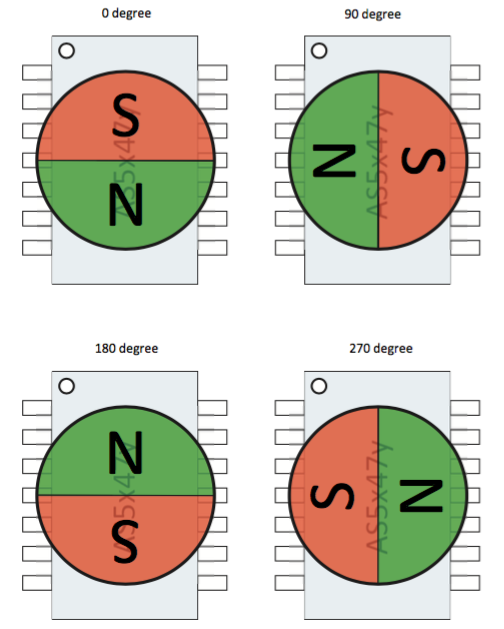
\includegraphics[height=4in]{figures/magnetic_field.png}

    \caption[Magnet and AS5047D]{Magnet and AS5047D \citep{1}}

    \label{magnet_rotation}
\end{center}
\end{figure}

\subsection{Motorlab Parts}
\label{makereference2.1.2} 

Along with the hardware mentioned in section ~\ref{makereference2.1.1}, three components were needed to be developed in order to bring the Motorlab to fruition: a printed circuit board that houses the on-axis magnetic rotary position sensor, a spacer to put distance between the circuit board and the motor, and a magnet holder, which holds one diametrically opposed magnet ~\footnote{Diametrically opposed meaning the north and south poles of the magnet are in-plane as opposed to top/bottom poles. Reference figure ~\ref{magnet_rotation} for further clarification}. Both the spacer and magnet holder which can be seen in figure \ref{section_view_motorlab} had to be 3D printed in order to achieve the required specifications of the apparatus setup. Detailed drawings of these two parts can be found in (appendix) if reproduction is desired. Along with the two 3D printed parts, a printed circuit board had to be designed by Eric Patterson of Kansas State University to allow the position sensor to communicate with the rest of the hardware.

Because of variability in resolution of current 3D printers, care was given to the design of the magnet holder. A spline was used for both the shaft of the magnet holder and the section that holds the magnet itself. The spline allowed for greater tolerances in the parts, meaning the magnet holder could be easier to press fit into the motor, and likewise allowed easier removal of the diametrically opposed magnet.

\begin{figure}[htb]%t=top, b=bottom, h=here

    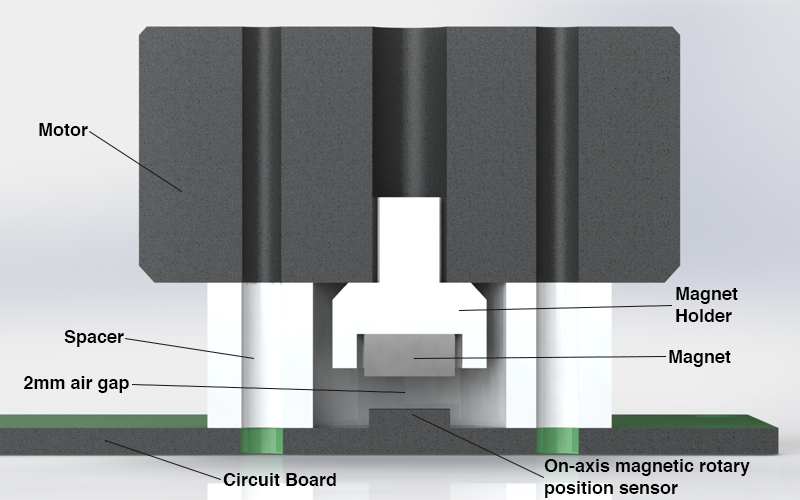
\includegraphics[height=4in]{figures/section_view_motorlab_assembly.png}

    \caption[Section View of Motorlab Assembly]{Section View of Motorlab Assembly}

    \label{section_view_motorlab}
\end{figure}


\section{Motorlab}
\label{makereference2.2} 

Need information here